\section{Présentation du projet}

\subsection{Énoncé}
Lorsque nous avons sélectionné notre projet, l'énoncé d'origine était le suivant : \\
\enquote{Étant donné un échiquier de dimension $m \times n$, énumérer tous les circuits hamiltoniens réalisés en utilisant uniquement les mouvements du cavalier dans le jeu d'échecs. Même question, mais en énumérant le nombre de chemins hamiltoniens "ouverts" (origine et destination différentes).}

A cet énoncé, nous avons décidé d'ajouter une autre partie : \\
\enquote{Étant donné un échiquier de dimension $m \times n$, générer et afficher un circuit (ou un chemin) hamiltonien basé uniquement sur les mouvements du cavalier.}
\subsection{Les bases du problème du cavalier}
Le problème du cavalier peut donc être représenté sous la forme d'un graphe. Chaque case de l'échiquier est un sommet et chaque mouvement possible à partir de cette case vers une autre case est une arête du graphe.

\begin{figure}[h]
\begin{center}
   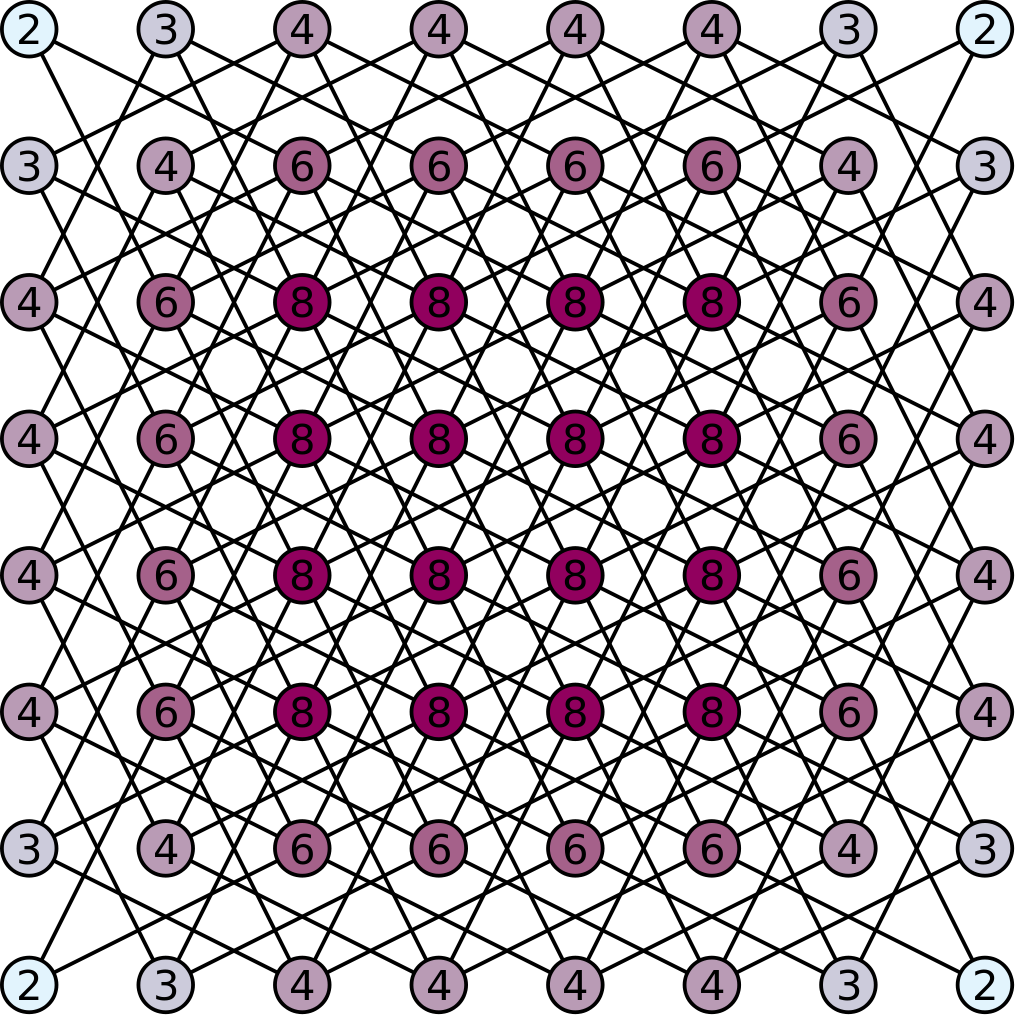
\includegraphics[scale=0.18]{img/graph_cavalier.png} 
   \caption{\label{cavalier_graphe} Graphe du cavalier sur un échiquier $8 \times 8$(inclure source ici wiki)}
   \end{center}
\end{figure}

Le graphe de la figure ~\ref{cavalier_graphe} représente les déplacements possibles pour un cavalier sur un échiquier classique. Le chiffre attribué à chaque case représente le nombre de cases accessibles en un mouvement depuis celle-ci. La réalisation de ce travail implique la génération d'un graphe similaire, généralisé à n'importe quelle taille $m \times n$. 

Le graphe ainsi généré peut ensuite être exploité pour y trouver des chemins et circuits hamiltoniens.

